\documentclass[10 pt]{amsart}
\usepackage{amscd,amsmath,amsthm,amssymb}
\usepackage{enumerate,varioref}
\usepackage{epsfig}
\usepackage{graphicx}
\usepackage{mathtools}
\usepackage{tikz}
\usepackage{lscape}
\newtheorem{thm}{Theorem}
\newtheorem{cor}[thm]{Corollary}
\newtheorem{lem}[thm]{Lemma}
\newtheorem{prop}[thm]{Proposition}
\theoremstyle{definition}
\newtheorem{defn}[thm]{Definition}
\theoremstyle{remark}
\newtheorem{ex}[thm]{Example}
\newtheorem{rem}[thm]{Remark}
\numberwithin{equation}{subsection}
\newcommand{\R}{\mathbb{R}}
\newcommand{\Z}{\mathbb{Z}}
\newcommand{\C}{\mathbb{C}}
\newcommand{\Q}{\mathbb{Q}}
\newcommand{\B}{\textbf}

\begin{document}

\title{Proof of Can-USA-Mex Graph Unable to be Represented by Three Colors}
\author{}

\email{} \maketitle

\section*{Claim}
Because the Can-USA-Mex Graph contains the graph shown below, three\newline coloring is impossible.
%\begin{landscape}
\[
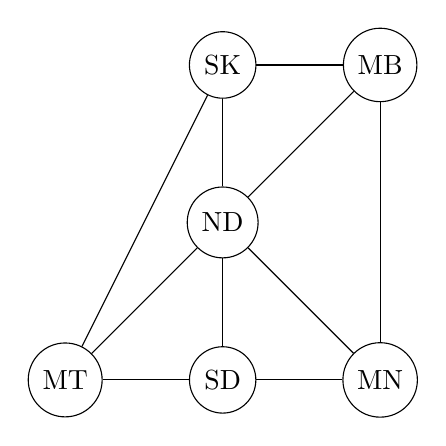
\begin{tikzpicture}
\node[circle, draw] (MT) at (0,0){MT};
\node[circle, draw] (SK) at (2,4){SK};
\node[circle, draw] (ND) at (2,2){ND};
\node[circle, draw] (SD) at (2,0){SD};
\node[circle, draw] (MB) at (4,4){MB};
\node[circle, draw] (MN) at (4,0){MN};
\foreach \from/\to in 
{MT/SK,MT/ND,MT/SD,SK/ND,SK/MB,MB/ND,MB/MN,ND/SD,ND/MN,SD/MN}
\draw (\from) -- (\to);
\end{tikzpicture}
\]
%\end{landscape}
\section*{Proof}
\begin{proof}
Let the graph we want to three color be made up of nodes 1 thorugh 6,\newline topologically congruant to the graph in the claim, and connected as such:
%\begin{landscape}
\[
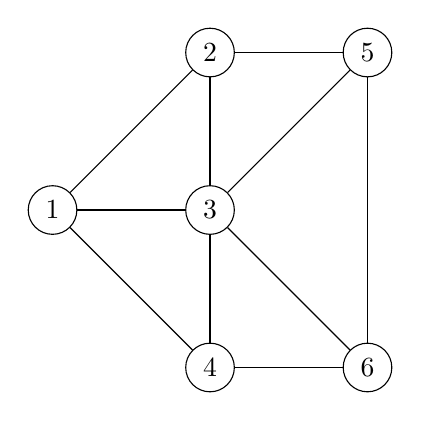
\begin{tikzpicture}
\node[circle, draw] (1) at (0,2){1};
\node[circle, draw] (2) at (2,4){2};
\node[circle, draw] (3) at (2,2){3};
\node[circle, draw] (4) at (2,0){4};
\node[circle, draw] (5) at (4,4){5};
\node[circle, draw] (6) at (4,0){6};
\foreach \from/\to in 
{1/2,1/3,1/4,2/3,2/5,5/3,5/6,3/4,3/6,4/6}
\draw (\from) -- (\to);
\end{tikzpicture}
\]
%\end{landscape}
Because nodes 2 and 4 are both connected to nodes 1 and 3, regardless of the colors of nodes 1 and 3, nodes 2 and 4 must be the same color.
\newline
\newline
In this case, node 1 will be blue, node 3 will be red, and nodes 4 and 2 will be orange. Notice how no two adjacent nodes share the same color.
%\begin{landscape}
\[
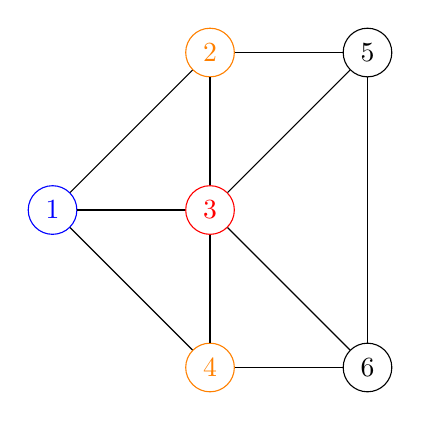
\begin{tikzpicture}
\node[circle, draw, color=blue] (1) at (0,2){1};
\node[circle, draw, color=orange] (2) at (2,4){2};
\node[circle, draw, color=red] (3) at (2,2){3};
\node[circle, draw, color=orange] (4) at (2,0){4};
\node[circle, draw] (5) at (4,4){5};
\node[circle, draw] (6) at (4,0){6};
\foreach \from/\to in 
{1/2,1/3,1/4,2/3,2/5,5/3,5/6,3/4,3/6,4/6}
\draw (\from) -- (\to);
\end{tikzpicture}
\]
%\end{landscape}
Because nodes 3 and 4 are red and orange respectively, and are also both connected to node 6, node 6 must be the third color, blue.
%\begin{landscape}
\[
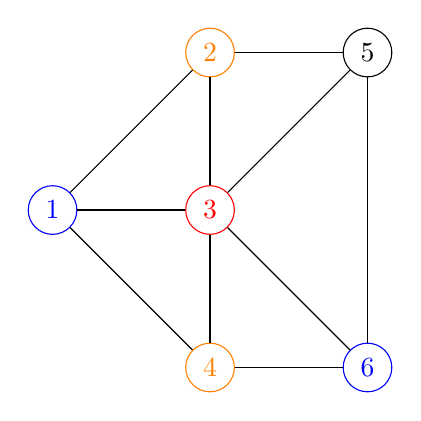
\begin{tikzpicture}
\node[circle, draw, color=blue] (1) at (0,2){1};
\node[circle, draw, color=orange] (2) at (2,4){2};
\node[circle, draw, color=red] (3) at (2,2){3};
\node[circle, draw, color=orange] (4) at (2,0){4};
\node[circle, draw] (5) at (4,4){5};
\node[circle, draw, color=blue] (6) at (4,0){6};
\foreach \from/\to in 
{1/2,1/3,1/4,2/3,2/5,5/3,5/6,3/4,3/6,4/6}
\draw (\from) -- (\to);
\end{tikzpicture}
\]
%\end{landscape}
Because nodes 2 and 4 are the same color, orange, and nodes 2 and 3 are connected to node 5, node 5 must also be the third color, blue.
%\begin{landscape}
\[
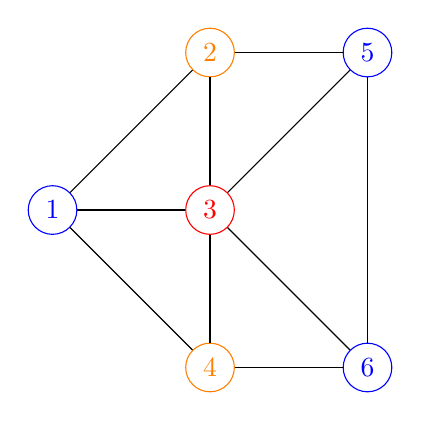
\begin{tikzpicture}
\node[circle, draw, color=blue] (1) at (0,2){1};
\node[circle, draw, color=orange] (2) at (2,4){2};
\node[circle, draw, color=red] (3) at (2,2){3};
\node[circle, draw, color=orange] (4) at (2,0){4};
\node[circle, draw, color=blue] (5) at (4,4){5};
\node[circle, draw, color=blue] (6) at (4,0){6};
\foreach \from/\to in 
{1/2,1/3,1/4,2/3,2/5,5/3,5/6,3/4,3/6,4/6}
\draw (\from) -- (\to);
\end{tikzpicture}
\]
%\end{landscape}
This isn't allowed in three coloring because nodes 5 and 6 share the same color, and are also adjacent to eachother.
\newline
\newline
Because of this, the graph cannot be three colored.
\newline
Therefore the Can-USA-Mex Graph can not be three colored either.
\end{proof}
\end{document}